\documentclass[12pt]{article}
\usepackage[longnamesfirst]{natbib}
% \usepackage{color} option clash
\usepackage{graphicx}
% \usepackage[dvips]{graphics}

\input{../standard}
\newtheorem{definition}{Definition}

% --- Paragraph split
\setlength{\parskip}{0.00in}

% --- Line spacing
\renewcommand{\baselinestretch}{1.4}

% --- Margin notes on the left-hand-side
%    \marginpar{\scriptsize\raggedright note}
\setlength{\topmargin}{0in}         % 1.5 in top/bottom
\setlength{\headheight}{0.25in}
\setlength{\headsep}{0.25in}
\setlength{\textheight}{8.0in}
\setlength{\oddsidemargin}{0.0in}   % 1. in left/right
\setlength{\textwidth}{6.5in}

% --- Hypthenation
\sloppy  % fewer hyphenated
\hyphenation{stan-dard}
\hyphenation{among}

% --- Customized commands, abbreviations
\newcommand{\TIT}{{\it  {\tiny  Alpha-investing}}}
\newcommand{\SDR}[1]{{\mbox{$\mbox{SDR}_{\mbox{\scriptsize #1}}$}}}

% --- Header
\pagestyle{myheadings}
\markright{\TIT}

\usepackage[usenames]{color}

\newcommand{\jrss}[1]{\noindent{\textcolor{red}{\{{\bf jrss:} \em
#1\}}}}
\newcommand{\dpf}[1]{\noindent{\textcolor{blue}{\{{\bf dpf:} \em
#1\}}}}
\newcommand{\ras}[1]{\noindent{\textcolor{green}{\{{\bf ras:} \em
#1\}}}}


% --- Title

\title{  
\vspace{-0.5em}
         Alpha-investing: A new multiple hypothesis testing procedure
         that controls mFDR 
\vspace{-0.5em}
}
% \title{  
%        Multiple hypothesis testing using \\
%        the excess discovery count and alpha-investing rules
% }

\author{
        Dean P. Foster and Robert A. Stine\footnote{All correspondence
regarding this manuscript should be directed to Prof. Stine at 
the address shown with the title.  He can be reached via e-mail at
stine@wharton.upenn.edu.}                                    \\
        Department of Statistics                             \\
        The Wharton School of the University of Pennsylvania \\
        Philadelphia, PA 19104-6340                          \\
}

\date{\today}
% \date{April 7, 2005}

%%%%%%%%%%%%%%%%%%%%%%%%%%%%%%%%%%%%%%%%%%%%%%%%%%%%%%%%%%%%%%%%%%%%%%%%%%%

\begin{document}
\maketitle 
%------------------------------------------------------------------------
\vspace{-2em}

\abstract{ 
\vspace{-0.5em}
We propose alpha-investing for testing multiple hypotheses.  
 Alpha-investing is an adaptive, sequential methodology that encompasses a
 large family of procedures. All control mFDR, which is the ratio of
 the expected number of false rejections to the expected number of
 rejections. mFDR is a weaker criterion than FDR, which is the
 expected value of the ratio.  We compensate for this weakness by
 showing that alpha-investing controls mFDR at every rejected
 hypothesis.  Alpha-investing resembles alpha-spending used
 in sequential trials, but possess a key difference.  When a test
 rejects a null hypothesis, alpha-investing earns additional
 probability toward subsequent tests.  Alpha-investing hence allows one
 to incorporate domain knowledge into the testing procedure and
 improve the power of the tests. In this way, alpha-investing
 enables the statistician to design a testing procedure for a specific problem 
 while guaranteeing control of mFDR.  }

%------------------------------------------------------------------------
\vspace{0.05in}

\noindent
{\it Key words and phrases: 
  Bonferroni method,
  false discovery rate (FDR, mFDR), 
  family wide error rate (FWER),
  multiple comparison procedure.
}



 
% ----------------------------------------------------------------------
\section{Introduction}                                   %  1
% ----------------------------------------------------------------------
\label{sec:introduction}

We propose an adaptive, sequential methodology for testing multiple
hypotheses. Our approach, called alpha-investing, works in the usual
setting in which one has a batch of several hypotheses as well as
cases in which the hypotheses arrive sequentially in a stream.
Streams of hypotheses arise naturally in variety of contemporary
modeling applications, such as genomics and variable selection for
large models.  In contrast to the comparatively small problems that
spawned multiple comparison procedures, modern applications can
involve thousands of tests.  For example, micro-arrays lead one to
compare a control group to a treatment group using measured
differences on over 6,000 genes \citep{shaffer03}.  If one considers
the possibility for interactions, then the number of tests is
virtually infinite. In contrast, the example used by Tukey to motivate
multiple comparisons compares the means of only 6 groups
\citep[][available in \citet{braun94}] {tukey53}.  Because
alpha-investing allows the testing to proceed sequentially, the choice
of future hypotheses can depend upon the results of previous tests.
Thus, having discovered differences in certain genes, an investigator
could, for example, direct attention toward genes that share common
transcription factor binding sites \citep{gupta05}.

Before we describe alpha-investing, we introduce a slight variation on
 the marginal false discovery rate (mFDR), a existing criterion for
 multiple testing.  mFDR is defined as follows. Let the observable
 random variable $R$ denote the total number of hypotheses rejected by
 a testing procedure, and let $V$ denote the unobserved number of
 falsely rejected hypotheses.  Ideally $V$ is small.  Then controlling
 a version of mFDR, which we denote mFDR${}_1$, at level $\alpha$ means
\begin{equation}
\label{eq:mFDR}
\hbox{mFDR}_1 \equiv \frac{E(V)}{E(R) + 1} \le \alpha.
\end{equation}
mFDR traditionally does not add 1 to the denominator; following our
notation, we denote the traditional version mFDR${}_0$. The notation
mFDR${}_1$ will remind purists that this isn't exactly the usual
definition.  The addition of a positive constant to the denominator
avoids statistical problems under the complete null.  Under the
complete null, all hypotheses are false.  In this case, $V \equiv R$
and mFDR${}_{0}$ = 1 for all procedures.  We contrast mFDR${}_0$ with
$\hbox{FDR} \equiv E(V/R)$ after we introduce alpha-investing.

An alpha-investing rule is an adaptive testing procedure. In what
follows, we show that all alpha-investing rules control mFDR${}_1$.
Alpha-investing rules generalize alpha-spending rules.  An
alpha-spending rule begins with an initial allowance for Type I error,
what we call the initial alpha-wealth of the procedure.  Each test at
level $\alpha_i$ reduces the alpha-wealth of the spending rule by
$\alpha_i$.  Once the alpha-wealth of the spending rule reaches zero,
no further tests are allowed.  Alpha-spending natually implements a
Bonferroni rule.  By the union rule of probability, the total chance
of making a Type I error is bounded by the intial alpha-wealth.  In
multiple testing, however, Bonferroni rules are too conservative.  We
invented alpha-investing rules to overcome this conservatism.

We escape the conservatism of Bonferroni rules in the following
 way. Each time an alpha-investing rule rejects a null hypothesis, it
 earns a contribution to its alpha-wealth.  Thus rejections beget more
 rejections.  This idea of alpha-wealth begetting more alpha-wealth
 leads us to call this class of procedures alpha-investing
 rules. Alpha-investing rules allow one to test a possibly infinite
 stream of hypotheses, accommodate dependent tests, and incorporate
 domain knowledge.  Like alpha-spending rules alpha-investing rules
 free the statistician to allocate the available Type I error among the
 various hypotheses, all the while protecting from
 excessive false rejections.

The sequential nature of alpha-investing allows us to enhance the
 type of control obtained through mFDR. Though mFDR is successful
 in identifying good multiple testing procedures, it is often compared
 unfavorably to the more famous FDR.  Both FDR and mFDR${}_0$ were suggested
 in \citet{benjamini95} along with mFDR${}_1$, which they considered
 somewhat artificial. After all, mFDR does not control a property of
 the realized sequence of tests, instead controlling a ratio of
 expectations over the ensemble of test sequences. In contrast, FDR
 controls the expectation of $V/R$ for a given sequence.  Nonetheless,
 FDR does not produce the type of control we would like.  Ideally we
 would like to be guaranteed that at the point we reject $k$
 hypotheses, at most $.05\,k$ of these have been incorrectly rejected
 on average.  Neither FDR, nor mFDR, permit such claims.

By placing mFDR in a sequential setting, we can require that a
 procedure do well if stopped early.  Suppose rather than testing all
 $m$ hypotheses, the statistician stops after rejecting 10.
  We would like to be able to assure her that no more than, say, 2 of
 these were false rejections, on average.  This further control distinguishes
 what we describe as ``uniform control'' of mFDR.

Suppose we test hypotheses until the total number of rejections $R$
reaches some target $r$.  Let $T_{r}$ identify the index of this test.
Define $V(T_{r})$ to be the number of nulls that have been incorrectly
rejected at this point. A test procedure uniformly controls
mFDR${}_{1}$ if this stopped process controls mFDR${}_{1}$ in the
sense of (\ref{eq:mFDR}). In words, equation (\ref{eq:mFDR}) shows
that the expected value of $V_R$ given that $R=r$ is less than or
equal to $\alpha(r+1)$.  This conditional expectation requires that we
introduce a stopping time which stops the testing procedure when
$R=r$.  We leave these details for section \ref{sec:sFDR}.  As a
preview of our results, we give the following theorem:
\begin{theorem}\label{thm:stopped}
An alpha-investing rule with control parameters set to $\alpha$ has
 the property that $E \; V(T_{r}) \le \alpha(r+1)$ where $T_{r}$ is
 the stopping time defined by occurrence of the $r^{th}$ rejection, and
 $V(m)$ is the number of false rejections when $m$ hypothesis have
 been tested.
\end{theorem}
In fact, when a sequence of tests is stopped at a fixed number of rejections,
 many of the variations on FDR are equivalent (see Theorem
 \ref{thm:all:same}.)

The rest of this paper develops as follows.  We first review several
 ideas from the literature on multiple comparisons, particularly those
 related to the familywise error rate and FDR.  Next we discuss
 alpha-investing rules in Section \ref{sec:alpha:investing}.  In
 sections \ref{sec:mFDR} and \ref{sec:sFDR} we discuss uniform control
 of mFDR.  In Section \ref{sec:results}, we show that alpha-investing
 rules uniformly control mFDR.  We describe the design of
 alpha-investing rules and give several examples in Section
 \ref{sec:examples}.  We close in Section \ref{sec:discussion} with a
 brief summary.  We generally defer proofs to the appendix.


%--------------------------------------------------------------------------
\section{Criteria and Procedures }  \label{sec:procedure} % 2
%--------------------------------------------------------------------------

To set the stage for describing alpha-investing and our modification
of mFDR, we review the two criteria most commonly applied in testing
multiple hypotheses: the family-wise error rate and the false
discovery rate.  These criteria generalize the notion of the Type I
error rate ($\al$-level) to tests of several hypotheses.  Just as
there are many $\al$-level tests of a simple hypothesis, so too are
there various procedures for testing multiple hypotheses.  We confine
our review to two: the Bonferroni rule (as implemented using
alpha-spending) and step-down tests.  These two are closely related to
the alpha-investing rules described in Section
\ref{sec:alpha:investing}.

Suppose that we have a set of $m$ null hypotheses ${\cal H}(m) =
\{H_1, \, H_2, \ldots, H_m\}$ that specify values for parameters
$\theta = \{\theta_1,\,\theta_2, \ldots, \theta_m \}$.  Each parameter
$\theta_j$ can be scalar or vector-valued, and $\Theta$ denotes the
space of parameter values.  In the most familiar case, each null
hypothesis specifies that a scalar parameter is zero, $H_j: \theta_j =
0$.  We describe the situation in which every null hypothesis is true
as the ``complete null hypothesis.''

We follow the standard notation for labeling the true and false
rejections \citet{benjamini95}.  Assume that $m_0$ of the null
hypotheses in ${\cal H}(m)$ are true.  The {\em observable} statistic
$R(m)$ counts how many of these $m$ hypotheses are rejected.  The {\em
  unobservable} random variable $V^\theta(m)$ denotes the number of
false positives among the $m$ tests, those cases in which the testing
procedure incorrectly rejects a true null hypothesis.  Similarly,
$S^{\theta}(m) = R(m)-V^\theta(m)$ counts the number of correctly
rejected null hypotheses.  We index these random variables with a
superscript $\theta$ to distinguish them from a statistic such as
$R(m)$; $V^\theta(m)$ and $S^\theta(m)$ are not observable without
$\theta$.  For the complete null hypothesis, $m_0 = m$, $V^\theta(m)
\equiv R(m)$ and $S^{\theta}(m) \equiv 0$.

The original intent of multiple testing was to control the chance for {\em
any} false rejection.  The {\em family-wise error rate} (FWER) is the
probability of falsely rejecting {\em any} null hypothesis from ${\cal
H}(m)$, regardless of the underlying parameters,
\begin{equation}
  \mbox{FWER}(m) \equiv 
   \sup_{\theta \in \Theta} \pr_\theta(V^\theta(m) \ge 1) \;.
\label{eq:fwer}
\end{equation}
An important special case is control of FWER under the complete null
 hypothesis:
\begin{equation}
 \pr_0(V^\theta(m) \ge 1) \le \alpha \;,
\label{eq:size}
\end{equation}
where $\pr_0$ denotes the probability measure under the complete null
 hypothesis.  We refer to this goal as controlling FWER in the weak
 sense.  All of the procedures that we describe control FWER in the
 weak sense, but not all control FWER more generally.

The Bonferroni procedure is familiar and represents an important
benchmark for comparison.  Let $p_1, \ldots, p_m$ denote the p-values
of tests of $H_1, \ldots, H_m$.  Given a chosen level $0 < \alpha < 1$,
the usual Bonferroni procedure rejects those $H_j$ for which $p_j \le
\al/m$.  Let the indicators $V^\theta_j \in \{0, 1\}$ track incorrect
rejections; $V^\theta_j = 1$ if $H_j$ is incorrectly rejected and is
zero otherwise.  Then $V^\theta(m) = \sum V^{\theta}_{j}$ and the
inequality
\begin{equation}
  \pr_\theta(V^\theta(m) \ge 1) 
     \le \sum_{j=1}^m \pr_\theta(V^{\theta}_{j} = 1) \le \al
\label{eq:Bon}
\end{equation}
shows that the traditional Bonferroni procedure controls
$\mbox{FWER}(m) \le \alpha$.  One need not distribute $\alpha$ equally
over ${\cal H}(m)$; the inequality \eqn{eq:Bon} requires only that the
sum of the $\alpha$-levels not exceed $\alpha$.  This observation
suggests the alpha-spending characterization of the Bonferroni
procedure.  As an alpha-spending rule, the Bonferroni procedure
allocates $\alpha$ over a collection of hypotheses, devoting a larger
share to hypotheses of greater interest.  In effect, the procedure has
a budget of $\alpha$ to spend.  It can spend $\alpha_j \ge 0$ on
testing each hypothesis $H_j$ so long as $\sum_j \alpha_j \le \alpha$.
Although such alpha-spending rules control FWER, they are often
criticized for having little power.  Clearly, the power of the
traditional Bonferroni procedure decreases as $m$ increases because
the threshold $\alpha/m$ for detecting a significant effect decreases.
The testing procedure introduced in \citet{holm79} offers more power
while controlling FWER, but the improvements are small.
 

To obtain substantially more power for multiple testing,
\citet{benjamini95} introduced a different criterion, the false
discovery rate (FDR).  A procedure that controls FDR also controls
FWER in the weak sense.  If the complete null hypothesis is rejected,
however, FDR introduces a different type of control on the testing
procedure.  \citet{benjamini95} defines FDR as the expected proportion
of false positives among rejected hypotheses,
\begin{equation}
  \mbox{FDR}(m) = E_\theta \left(\frac{V^\theta(m)}{R(m)} \given R(m)>0 \right)
               \pr (R(m)>0)  \;.
\label{eq:fdr}
\end{equation}
For the complete null hypothesis, $R(m) \equiv V^\theta(m)$ and
$\mbox{FDR}(m) = \pr_0(R(m)>0)$, which is just $\mbox{FWER}(m)$.
Thus, test procedures that control FDR$(m) \le \alpha$ control the
FWER$(m)$ in the weak sense at level $\alpha$.  Under the alternative,
$\mbox{FDR}(m)$ decreases as the number of false null hypotheses
$m-m_0$ increases \citep{shaffer03}.  As a result, $\mbox{FDR}(m)$
becomes more easy to control in the presence of non-zero effects,
allowing more powerful procedures.  Variations on FDR include pFDR
\citep[which drops the term $\pr (R>0)$][]{storey02,storey03} and the
local false discovery rate $\mbox{fdr}(z)$ \citep[which estimates the
  false discovery rate as a function of the size of the test
  statistic][]{efron04, efron05}.  Closer to our work,
\citet{rice06} and \citet{meinshausen04b} consider estimates
of $m_0$, the total number of false hull hypotheses in ${\cal H}(m)$.


\citet{benjamini95} also introduces a step-down testing procedure that
 controls FDR. Order the collection of $m$ hypotheses so that
 the p-values of the associated tests are sorted from
 smallest to largest (putting the most significant first),
\begin{equation}
  p_{(1)} \le p_{(2)} \le \cdots \le p_{(m)} \;.
\label{eq:ordered:pv}
\end{equation}
The test of $H_{(1)}$ has p-value $p_{(1)}$, the test of $H_{(2)}$ has
p-value $p_{(2)}$ and so forth.  The step-down procedure of
\citet{benjamini95} (BH) first compares the smallest p-value to the
Bonferroni threshold.  If $p_{(1)} > \alpha/m$, the BH procedure stops
and does not reject any hypothesis.  This step controls {\em FWER} in
the weak sense at level $\alpha$.  If $p_{(1)} \le \alpha/m$, the
procedure rejects $H_{(1)}$ and moves on to $H_{(2)}$.  Rather
than compare $p_{(2)}$ to $\alpha/m$, however, the BH procedure
compares $p_{(2)}$ to a larger threshold, $2 \alpha/m$.  In general,
if we define $j_d = \min\{j:p_{(j)} > j\alpha / m\}$, then the BH
step-down procedure rejects $H_{(1)}, \ldots, \, H_{(j_d - 1)}$.
Clearly this sequence of larger thresholds produces more power than obtained by a Bonferroni procedure.  If
the p-values are independent, the inequality of \citet{simes86}
implies that this step-down procedure satisfies FDR. (This theorem was
first proved by \citet{benjamini95} who used a different proof.) This series of
thresholds, however, does not control FWER$(m)$ in general.  This is
the price we pay for the improvement in power.  Subsequent papers
\citep[such as][]{benjamini01, sarkar98, troendle96} consider
situations in which step-down testing controls FDR under certain types
of dependence.

%--------------------------------------------------------------------------
\section{Alpha-Investing Rules}   \label{sec:alpha:investing}         %   4
%--------------------------------------------------------------------------

Alpha-investing introduces a framework for devising multiple
 testing procedures that control mFDR in a dynamic setting that allows
 streams of hypotheses.  Alpha-investing resembles alpha-spending
 as used in sequential clinical trials.  In a
 sequential trial, investigators routinely monitor the accumulating
 results for safety and efficacy.  This monitoring leads to a sequence
 of tests of one (or perhaps a few) null hypotheses as the data
 accumulate.  An alpha-spending (or error-spending) rule controls the
 level of such tests.  Given an overall Type I error rate for the
 trial, say $\al = 0.05$, an alpha-spending rule allocates, or spends,
 $\alpha$ over a sequence of tests.  As \citet{tukey91} writes, ``Once
 we have spent this error rate, it is gone.''  When repeatedly testing
 one null hypothesis $H_0$ as data accumulate, alpha-spending
 guarantees that $P(\mbox{reject } H_0) \le \alpha$ when $H_0$ is true.

% The data might accumulate as additional patients enroll
% \citep{armitage69, demets94} or as more longitudinal data accrue
% \citep{tsiatis96}.  

While similar in that they allocate Type I error over multiple tests,
 alpha-investing differs from alpha-spending in the
 following way.  An alpha-investing rule earns additional probability
 toward subsequent Type I errors with each rejected hypothesis.
  Rather than treat each test as an expense that consumes its Type
 I error rate, an alpha-investing rule treats tests as investments,
 motivating our choice of name.  In keeping with this analogy, we call
 the Type I error rate available to the rule its alpha-wealth.  As
 with an alpha-spending rule, an alpha-investing rule can never spend
 more than its current alpha-wealth.  Unlike an alpha-spending rule,
 however, an alpha-investing rule earns an increment in its
 alpha-wealth each time that it rejects a null hypothesis.  For alpha-investing, Tukey's remark becomes ``Rules that invest the error rate
 wisely earn more for further tests.''  A procedure that
 invests its alpha-wealth in testing hypotheses that are rejected
 accumulates additional wealth toward subsequent tests.  The more
 hypotheses that are rejected, the more alpha-wealth it earns.  If the
 test of $H_j$ is not significant, however, an alpha-investing rule
 loses the invested  $\alpha$-level and its alpha-wealth
 decreases.  The more wealth a rule invests in testing hypotheses that
 are not rejected, the less alpha-wealth remains for subsequent tests.


More specifically, an alpha-investing rule is a function $\cal I$ that
determines the $\alpha$-level for testing the next hypothesis in a
sequence of tests.  We assume an exogenous system external to the
investing rule determines the next hypothesis to test.  (Though not
part of the investing rule itself, this exogenous system can use the
sequence of rejections $R_j$ to pick the next hypothesis.)  An alpha-investing rule has two parameters: the initial
alpha-wealth and the amount earned (called the pay-out) when a null
hypothesis is rejected.  Let $W(k) \ge 0$ denote the alpha-wealth
accumulated by an investing rule after $k$ tests; $W(0)$ is the
initial alpha-wealth.  For example, one might conventionally set $W(0)
= 0.05$ or $0.10$.  At step $j$, an alpha-investing rule sets the
level $\alpha_j$ for testing $H_j$ up to its current alpha-wealth, 
 $0 \le \alpha_j \le W(j-1)$.  The level $\alpha_j$ for testing $H_j$
typically depends upon the sequence of prior outcomes.  Let $R_j \in \{0,1\}$ be a sequence of binary random variables denoting the outcome of testing $H_{j}$.  Define
\begin{equation}
   R_{j} = \left\{\begin{array}{cl}
       1, & \mbox{if } H_{j} \mbox{ is rejected }(\alpha_{j}>p_{j}),\mbox{ and } \\
       0, & \mbox{ otherwise.}
       \end{array} \right.
\label{eq:Rj}
\end{equation}
In general, an alpha-investing rule is a function of the initial wealth $W(0)$ and the string of prior test outcomes,
\begin{equation}
  \alpha_j = {\cal I}_{W(0)}(\{R_1,\, R_2, \ldots,R_{j-1}\}).
\label{eq:invest-rule}
\end{equation}


The outcome of testing $H_{1},\,H_{2},\,\ldots,H_{j}$ determines the alpha-wealth
$W(j)$ available for testing $H_{j+1}$.  Let $p_j$ denote the
p-value of the test of $H_j$.  If $p_j \le \alpha_j$, the test rejects
$H_j$.  In this case, the investing rule earns the pay-out $\omega$ which is
added to its alpha-wealth.  If $p_j > \alpha_j$, the procedure does not
reject $H_j$ and its alpha-wealth decreases by $\alpha/(1-\alpha)$, slightly more than the cost extracted in alpha-spending.  The change in the alpha-wealth is thus
\begin{equation}
  W(j) - W(j-1) =
   \left\{ \begin{array}{cc}
                \omega                            & \mbox{ if } p_j \le \alpha_j  \;,\cr
                 \alpha_j/(1-\alpha_{j})     & \mbox{ if } p_j > \alpha_j   \;.
           \end{array} \right.
\label{eq:Wm}
\end{equation}
If the p-value is uniformly distributed on [0,1], then the expected
 change in the alpha-wealth is $-(1 - \omega) \alpha_j$.  This suggests
 alpha-wealth decreases when testing a true null hypothesis. Other payment systems are possible; see the discussion in Section \ref{sec:discussion}.

In the next section, we show that such alpha-investing rules control mFDR${}_{1}$.  The initial
 alpha-wealth $W(0)$ controls the chance for rejecting the complete
 null hypothesis.  Under the complete null hypothesis, an
 alpha-investing rule resembles an alpha-spending rule when no
 hypothesis is rejected.  Hence, it controls the $\mbox{FWER} \le
 W(0)$ in the weak sense.  Results in the next section describe how the initial wealth $W(0)$ and pay-out $\omega$ lead to control of mFDR.
 Whereas $W(0)$ controls the probability of rejecting the complete null
 hypothesis, the pay-out $\omega$ controls how the alpha-investing
 rule performs once it rejects the complete null hypothesis.  
 
 The notion of compensation for rejecting a hypothesis captured in
 \eqn{eq:Wm} allows one to build context-dependent information into
 the testing procedure.  Suppose that the substantive context suggests
 that the first few hypotheses are likely to be rejected and that false hypotheses come in clusters.  In this
 instance, one might consider using an alpha-investing rule that invests heavily at the start and after each rejection, as illustrated  by the following rule.  Assume that the most recently rejected hypothesis is $H_{k^{*}}$.
  If false hypotheses are clustered, an alpha-investing rule should
 invest most of the available wealth $W(k^{*})$ to test $H_{k^{*}+1}$.  One rule that does this is, for $j>k^{*}$,
\begin{equation}
  {\cal I}_{W(0)}^{\omega}(R_1,\, R_2, \ldots,R_{j-1})
     = \frac{6}{\pi^2} \;\frac{W(k^{*})}{(j-k^{*})^2} \;.
\label{eq:I-sqr}
\end{equation}
This rule invests $6/\pi^2 \approx 0.6$ of its wealth in testing $H_1$
 or the null hypothesis $H_{k^{*}+1}$ that follows a rejected
 hypothesis.  The $\alpha$-level falls off rapidly if subsequent
 hypotheses are tested and not rejected. If the substantive insight is
 correct and the false hypotheses are clustered, then tests of
$H_1$ or $H_{k^{*}+1}$ represent ``good  investments.''  An example in Section 6 illustrates these ideas.


While it is relatively straightforward to devise investing rules, it
 may be difficult {\it a priori} to order the hypotheses in such a way
 that those most likely to be rejected come first.  Such an ordering
 relies on the specific situation.  Another complication is
 the construction of tests for which one can obtain the p-values that determine
 the alpha-wealth of an investing rule.  In
 order to show that a procedure controls mFDR, we require the test of
 $H_j$ to have the property that
\begin{equation}
  \forall \theta \in \Theta, \quad
  E_\theta(V^\theta_j \given R_{j-1},\,R_{j-2},\, \ldots, R_1)
  \le \alpha_j   \;.
\label{eq:alpham}
\end{equation}
An alternative statement is that for all $\theta \in H_j$,
 $P_\theta(R_j = 1 \given R_{j-1},\,R_{j-2},\, \ldots, R_1) \le \alpha_j$.
Either statement amounts to requiring that, conditionally on having
either accepted or rejected the prior $j-1$ hypotheses, the level of the test of
$H_j$ does not exceed $\alpha_j$.  The tests need not be independent.


\paragraph{Remark.}  
Alpha-investing requires that the test of $H_j$ maintain the
stated $\alpha$-level conditionally on the binary random variables $R_1$,
$R_2, \,\ldots, R_{j-1}$.  In particular, we note that the test is not
conditioned on the test statistic (such as a $z$-score) or parameter
estimate.  Adaptive testing in a group sequential trial
\citep[e.g.][]{lehmacher99} uses the information on the observed
$z$-statistic at the first look.  \cite{tsiatis03} show that using
this information leads to a less powerful test compared to traditional
group sequential tests that only use acceptance at the first
look.

%--------------------------------------------------------------------------
\section{mFDR}   \label{sec:mFDR}                          % 5
%--------------------------------------------------------------------------

Since we are dealing with a sequence of hypothesis, we define a sequence of evaluations of mFDR.  The following definition also generalizes our subscript 1 on mFDR to an arbitary value.  
\begin{definition} Consider a procedure that sequentially tests
 hypotheses $H_{1},\, H_{2},\ldots$, where the hypothesis
 tested at time $m$ can depend on the previous test results.  Then we define
\begin{equation}
  \mbox{mFDR}_{\eta}(m) 
   = \sup_{\theta \in \Theta} \;
\frac{E_\theta[V^\theta(m)]}{E_\theta[R(m)] + \eta}  \;.
\label{eq:def:mFDR}
\end{equation}
A multiple testing procedure {\em controls mFDR${}_{\eta}(m)$ at level $\alpha$} if
 mFDR$_{\eta}(m) \le \alpha$.
\end{definition}
We typically set $\eta$ to either $1$ or  $1-\alpha$.  Values of $\eta$ near zero produce a less satisfactory criterion since under the complete null hypothesis,
no system can generate an mFDR${}_{0}$ better than 1.0 since $V^{\theta}(m) \equiv R(m)$.  

Control of mFDR${}_\eta$ can be used to insure control of FWER
 in the weak sense.  Under the complete null hypothesis
 $V^\theta(m) \equiv R(m)$ so that 
\begin{displaymath}
   E_\theta(V^\theta(m)) \le \frac{\alpha\;\eta}{1 - \alpha} \;.
\end{displaymath}
For $\eta = 1-\alpha$, this inequality shows that 
 $E_\theta(V^\theta(m)) \le \alpha$.  Hence control of mFDR$_{1-\alpha}$ implies control of FWER in the weak sense at level $\alpha$.

The following simulation  contrasts control of mFDR$_{\eta}$ with control of FDR.  
Figure \ref{fi:sim1} shows simulated values of FDR and
 mFDR for testing a collection of $m=200$ hypotheses using three
 procedures.  The test procedures are a naive, fixed-level test that rejects $H_j$ if $p_j \le  \al=0.05$, the standard Bonferroni procedure with $\alpha = 0.05/m$, and the step-down BH procedure.  The tested hypotheses $H_j: \mu_j = 0$ specify means
 of 200 normal populations.  We set the values of the $\mu_j$ by
 sampling a spike-and-slab mixture.  The mixture puts $100(1-\pi_1)$\%
 of its probability in a spike at zero; $\pi_1=0$ identifies the
complete null
 hypothesis.  The slab of this mixture -- the signal -- is a normal
 distribution, so that
\begin{equation}
   \mu_j \sim \left\{  \begin{array}{ccc}
                   0  &  w.p.  & 1-\pi_1 \cr
                   N(0,\sigma^2) & w.p. & \pi_1 
    \end{array} \right.  \;.
\label{eq:mu-j}
\end{equation}
We set the variance of the signal component of the mixture to
$\sigma^2 = 2 \log m$ so that the standard deviation of the non-zero
$\mu_j$ matches the bound commonly used in hard thresholding.  The
test statistics are independent, normally distributed random variables
$Z_j \iid N(\mu_j,1)$ for which the two-sided p-values are $p_j =
2(1-\Phi(|Z_j|))$.  Given these p-values, we computed FDR and
mFDR$_{1}$ in a simulation with 10,000 trials.  In the
simulation, we varied the amount of signal varying $\pi_1$ from 0 (the
complete null hypothesis) to 1.

\begin{figure}
\caption{\label{fi:sim1} \sl
FDR  and mFDR control FWER in the weak sense under the complete null hypothesis ($\pi_1=0$ with $\alpha = 0.05$) and as the number false null hypotheses increases.  The graphs show FDR (left) and mFDR (right,  $\eta = 1-\alpha$) for the
BH step-down procedure ($\cdots$), the standard Bonferroni procedure (---), 
and a naive procedure that rejects each hypothesis at level $\al=0.05$
($- \cdot -$).}

\vspace*{0.05in}
\centerline{ 
            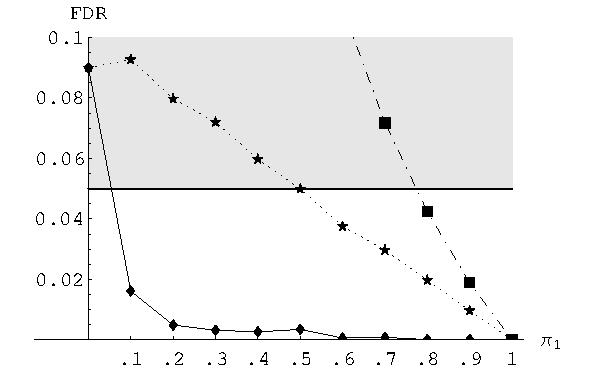
\includegraphics[width=3in]{fig_fdr}
            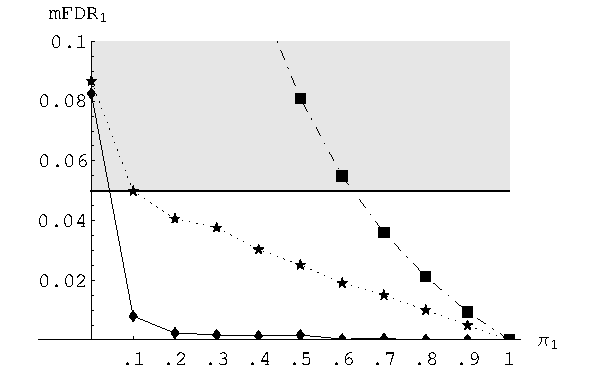
\includegraphics[width=3in]{fig_edc} 
           }

\end{figure}


Qualitatively, FDR and mFDR produce similar controls.  Both
criteria remain outside of the shaded regions for all values
 of $\pi_1$ for the BH step-down procedure and Bonferroni prcedures.   As $\pi_1$
 increases (and more hypotheses should be rejected), both FDR and mFDR fall toward zero.  \cite{shaffer03}
 discuss this aspect of FDR further.  Similarly, both criteria show the failures of the naive testing procedure; the criteria for the naive procedure that tests hypotheses at level 0.05 produces lie in the ``undesired''
 shaded region for all but the largest amounts of signal.  Both FDR and mFDR show
 this procedure as switching from liberal (shaded region) to
 conservative at about the same level of signal, namely $0.6 < \pi_1 <
 0.7$.   

%--------------------------------------------------------------------------
\section{Uniform control of mFDR}      \label{sec:sFDR}    % 5
%--------------------------------------------------------------------------

Alpha-investing allows one to test hypotheses sequentially, with the choice of the next hypothesis possibly dependent on prior outcomes.  Rather than begin with the full collection of ordered p-values, the testing proceeds one-at-a-time.  This flexibility allows the statistician to stop testing, for example, after the first rejected hypothesis.  To control a sequential testing procedure, we extend our definition of $mFDR_\eta(m)$ to random stopping times.  Recall the definition of a stopping time: $S$ is a stopping  time, if the event $S \le m$ can be determined by information known when the $m$th test is completed.  

\begin{definition}
 The mFDR${}_{\eta}(T)$ of a procedure for testing a stream of hypotheses
 $H_1,\,H_2,\, \ldots$ when the procedure is stopped at a stopping
time $T$ is
\begin{displaymath}
  \mbox{mFDR}_\eta(T) 
   = \sup_{\theta \in \Theta} \; \frac{E_\theta (V^\theta(T))}{E_\theta(R(T) ) + \eta }\;.
\end{displaymath}
\end{definition}

The supreme over all stopping times of our sequential definition of
mFDR will be called universal mFDR.
\begin{definition}
 A proceedure provides universal control of mFDR$_\eta$ at level $\alpha$ if 
\begin{equation}
\forall(T \in {\cal T}) \,\,  \mbox{mFDR}_\eta(T) \le \alpha
\label{eq:def:sFDR}
\end{equation}
where ${\cal T}$ is the set of bounded stopping times.
\end{definition}

Before we turn to proving that alpha-investing provides universal
 control of mFDR, let us first prove half of theorem
 \ref{thm:stopped}, namely any procedure that universally controls mFDR at
 level $\alpha$ can be thought of as having the conditional stopping
 property which we previous wrote as ``$E(V|R=r) \le \alpha(r+1)$.''
\dpf{We no longer use above notation}
\begin{definition}
Define the stopping time $T_{R=r} \equiv \inf_{t}\{t|R(t) = r\}$, where
 we take $T_{R=r}$ to be $\infty$ if the set is empty.
\end{definition}

\dpf{Should the following be a lemma instead of a theorem?}
\begin{theorem}
For any scheme which uniformly controls mFDR$_\alpha$ at level $\alpha$,
 we have that $E(V(T_{R=r})) \le \alpha (r + 1 - \alpha)$. 
\end{theorem}
{\bf Proof:}

We can stop the process at $T \equiv T_{R=r} \wedge \tau$ to make it
 a finite stopping time. Thus $E_\theta(R(T)) \le r$.  We know by
 our hypothesis $\frac{E_\theta ( V^\theta(T))}{E_\theta(R(T) ) +
 1 - \alpha } \le \alpha$ and so $E_\theta ( V^\theta(T)) \le
 \alpha(r+ 1 - \alpha)$.  Since this holds for all $\tau$, and
 $V^\theta(t)$ is bounded by $r$, we can take the limit to compute
 $E(V(T_{R=r})) \le \alpha(r+1 - \alpha)$.

\hfill \QED

\subsection{Relating mFDR to FDR}

mFDR and a variety of other modifications of FDR have been shown to be
 equivalent under a Bayesian setting (\cite{thc03}).  We will show
 that when stopped, all of these definitions are equivalent.

To start with, a bit of algebra shown in the appendix gives
\begin{equation}
0 \le \hbox{mFDR}_0 -  \hbox{FDR} -  \gamma_R \frac{\rho \sigma_V}{\mu_R} \le \gamma_R^2
\label{eq:bounds}
\end{equation}
where $\gamma_R = \sigma_R/\mu_R$, and $\rho$ is the correlation
 between $V$ and $R$.  When the coefficient of variation $\gamma_R$ is small, we see that 
 FDR and mFDR${}_0$ are close.

If $T_{r}$ is finite almost surely, then the standard deviation of
$R$ is identically zero, and hence $\gamma_R = 0$.  So, mFDR${}_0$ and FDR
are identical.

\begin{theorem}\label{thm:all:same}
Suppose $T_{r} < \infty$ almost surely.  Then the procedure that
 stops when exactly $r$ rejections have occured has the following properties:
\begin{enumerate}
\item $\gamma_R = 0$.
\item FDR = mFDR${}_1$ = cFDR = eFDR = pFDR = E(V)/r.
\item FDR$ \le \alpha \frac{r + 2}{r + 1}$ if the scheme controls the $sFDR_{0}$
 at level $\alpha$.
\end{enumerate}
\end{theorem}
{\bf Proof:}
Since $T_{r}$ is finite, we know that $R=r$ when we stop the
process.  Hence the standard deviation of $R$ is zero, and hence
$\gamma_R = 0$.  The second property follows from the various
definitions:
\begin{eqnarray*}
\hbox{FDR} &\equiv& E(V/R) = E(V)/r \\
\hbox{mFDR}_0 &\equiv& E(V)/E(R) = E(V) /r \\
\hbox{cFDR} &\equiv& E(V/R|R) =  E(V/R) = E(V)/r \quad \hbox{[almost surely]}\\
\hbox{eFDR} &\equiv& E(V)/R=  E(V)/r \quad  \hbox{[almost surely]}\\
\hbox{pFDR} &\equiv& E(V/R|R\ge 1) =  E(V/R) = E(V)/r \quad  \hbox{[almost surely]}
\end{eqnarray*}
and the fact that $R=r$ almost surely.  The third property follows by
 the definitions.

\hfill \QED

The above theorem is similar in spirit to \cite{thc03}.

If we restrict ourselves to alpha-investing rules with both $\omega$ and $W(0)$ set
 to $\alpha$ then it directly follows that
{\em
\begin{enumerate}\setcounter{enumi}{3}
\item $\Var(V) \le \alpha m$.
\item \label{itm:martingale} $P(V \ge 1 + \alpha m + k\sqrt{m}) \le e^{-k^2/2}$.
\end{enumerate}} 
%
Property \ref{itm:martingale} has a relationship to \cite{wasserman02} and
 \cite{wasserman04b}.  In \cite{wasserman04b} a stochastic process of
 hypothesis tests is considered.  Their approach contrasts with ours
 in that they use a stochastic process indexed by p-values, whereas we
 use one indexed by the apriori order that they are considered.  In
 both cases, an appropriate martingale is constructed that allows
 converting expectation results into tail probabilities.

It is not obvious that the condition of $T_{r} < \infty$ can in
 fact be met.  In the appendix, we explicitly construct a model
 for which this holds for many alpha-investing rules.  In
 fact, we will construct a class of such models with this property.  

\begin{theorem}\label{thm:finite:stopping}
There exists a model and an alpha-investing scheme such that $T_{r}$
 is almost surely finite for all $r$.
\end{theorem}

%--------------------------------------------------------------------------
\section{Alpha-Investing Rules Control mFDR}      \label{sec:results}    % 5
%--------------------------------------------------------------------------

This section discusses various procedures that control mFDR.    

We start by observing that it is always possible to construct a procedure for which mFDR$_{1} \le \alpha$.  Concrete examples are the Bonferroni procedure or alpha-spending.  The following theorem states that an alpha-investing rule ${\cal
 I}_{W(0)}^{\omega}$ with wealth determined by \eqn{eq:Wm} controls
 mFDR${}_{1-W(0)}$ so long as the pay-out $\omega$ is not too large.
  The theorem follows by showing that a stochastic process related to
 the alpha-wealth sequence $W(0), W(1), \ldots$ is a sub-martingale.
  Because the proof of this result relies only on the optional
 stopping theorem for martingales, we do not require independent
 tests, though this is the the easiest context in which to
 show that the p-values are honest in the sense required for
 \eqn{eq:alpham} to hold.

{\bf DEAN:  Check this.  It had a gamma before.  (It looks right.) }

\begin{theorem} \label{th:main} An alpha-investing rule ${\cal
 I}_{W(0)}^{\omega}$ governed by \eqn{eq:Wm} with initial alpha-wealth
 $W(0) \le \alpha \; \eta$ and pay-out $\omega \le \alpha$ controls
 mFDR$_\eta$ at level $\alpha$.
\label{eq:theorem1}
\end{theorem}
The above theorem also applies for the stopped version of mFDR.  A proof of the theorem is in the appendix.

%--------------------------------------------------------------------------
\section{Examples}              \label{sec:examples}           %  7
%--------------------------------------------------------------------------

The examples in this section illustrate alpha-investing.  We
 start with some general guidelines on how to construct
 alpha-investing rules.  Then we build a generic example using
 these rules.  Finally we will discuss how to construct an alpha-investing rule that is closely related to step-down procedures.

\subsection{Designing alpha-investing rules}

Alpha-investing frees the statistician to adapt the test procedure to the problem at hand.  Prior hopes and beliefs can be incorporated into the design of
 the procedure.  Patterns or structure among the hypotheses can
 also be incorporated.  It is even possible to change dynamically
 the order of testing the hypothesis.  Regardless of how these decisions are made, alpha-investing controls the mFDR.  The
 statistician is thereby given maximal freedom for making choices without
 landing in the quagmire of uncorrected multiplicities.  
 
This leaves the question of how these choices should be made.
We can recommend a few policies.   Whether none, several, or all of these
 suggestions are followed does not affect the applicability of our
 theorem that the mFDR will be controlled.   Instead of following
 these suggestions, the hypothesis could be tested in a random order with
 a fixed alpha-spending rule.

\paragraph{Best foot forward policy:} When using alpha-investing, it makes sense to test important hypotheses first.  There are two reasons for doing so.
 Ideally, the initial hypotheses include those we believe most likely to be
 rejected.  For example, in a testing drugs, it is common to
 test the primary endpoint before testing others.  The drug
 being tested has been designed to have its largest impact on primary
 endpoint.  The rejection of the leading hypotheses earns additional alpha-wealth toward tests of secondary endpoints.
 
 There is, however, a devious side to this policy that should be avoided. If ${\cal H}(m)$ is contaminated with trivially-false hypotheses to produce alpha-wealth, then all subsequent tests are tainted.  As an extreme example, suppose the first hypothesis is ``gravity does not exist.''  After rejecting this
 hypothesis, a procedure has more alpha-wealth to use in later tests than present in $W(0)$.  Most readers would, however, be uncomfortable using this additional alpha-wealth to test the primary endpoint of a drug.  In a sense, it is important to allow
an observer to ignore the list of tested hypotheses from some point onward. The design of the test procedure should then put the most interesting hypothesis first to insure that that when the reader stops, they have seen the most important results.  

\paragraph{Spending-rate policies:} Compared to ordering the hypotheses,
 deciding how much alpha-wealth to spend on each is relatively less important.  If
 a procedure spends its alpha-wealth too slowly, it will have alpha-wealth left at the end of the sequence of tests.  Since there is no
 reward  for leaving this alpha-wealth unused, the procedure could have used more powerful tests.  In this, spending at too slow a rate is inefficient.

Alternatively, spending too quickly means that the procedure may not have a chance to reject later hypotheses due to running out of
 alpha-wealth before reaching these.  It seems reasonable to save at
 least a small amount of alpha-wealth for the future.  

Spending-rate policies come in various forms.  The previous policies assume that the order of the hypotheses completely capture our beliefs: best first, worst last.   In other instances, it might be that hypotheses are clumped.  For example, hypotheses 10-20 might test the activity of one family of chemicals, and hypotheses 21-30 might test a different family. Once a rejection is made, it carries implications for the entire family.  In this case, it makes sense to use an alpha-investing rule that provides a burst of spending after a rejection is made in hopes that the next hypothesis is similar to the current hypothesis.   

\paragraph{Dynamic-ordering policies:} Suppose you are lucky enough to have a
 drug that might cure cancer {\em and} heart disease.  Clearly, these two
 hypotheses should come first on the list.  But what should come next?
  If the procedure rejects one of them but not the other, then the entire collection of subsequent tests depend on which one has been rejected.  The appropriate
 test to try next is very different in these cases.  We call a policy that adapts the order of the tests a dynamic ordering policy.  The nature of these policies is clearly domain-specific.  Besides encouraging such policies as good designs, we cannot give explicit suggestions as to how to implement these.

\paragraph{Revisiting policies:} Our theorems make no assumptions on how the various hypothesis are related.  This flexibility makes it possible to test  hypotheses that are very ``close'' to others.  In fact, our theorems
 hold even if the same hypothesis is tested more than once.  Of
 course, the second test must be conditional on the random variable $R_{j}$
 which represents the outcome of the first test.  We call this ``revisiting a
 hypothesis.''  For example, it might be sensible initially to test $H_{j}$
 at a small level $\alpha_{j} = 0.001$ (so as not to spend much alpha-wealth) and then test other hypotheses. If the test does not
 reject the first time, it might make sense to test it
 again at a higher level, say, 0.01.  In this way, the procedure can manage its alpha-wealth among a variety of
 hypotheses -- spending a little here and then a little spent there.  This policy
 is very useful in mimicking step-down testing.


\subsection{Example: Leveraging Domain Knowledge}

The performance of alpha-investing improves if the investigator ``knows the science.''  If the investigator is able to order hypotheses {\it a priori} so
that the procedure first tests those most likely to be rejected, then
alpha-investing can reject more hypotheses than the step-down test of Benjamini and Hochberg.  The full benefit is only realized, however, when one
exploits spending-rate policy. 

Suppose that the test procedure rejects $H_{k^{*}}$ and is about to
test $H_{k^{*}+1}$.  Rather than spread its current alpha-wealth
$W(k^{*})$ evenly over the remaining hypotheses, a rule can invest
more in testing the next hypothesis.  For example, one can allocate
$W(k^{*})$ using a discrete probability mass function such as this
version of the investing rule \eqn{eq:I-sqr}.  If none of the
remaining hypotheses are rejected, then the level for testing $H_j$ is
\begin{equation}
  \alpha_j
  = \frac{W(k^{*})}{h_{m-k^{*},2}} \; \frac{1}{(j-k^{*})^2}, \quad
    j = k^{*}+1,\ldots,m \;,
\label{eq:aggressive}
\end{equation}
where the normalizing constant $h_{q,2} = \sum_{i=1}^q 1/i^2$.  If one
of these tests rejects a hypothesis, the procedure reallocates its
wealth so that all is spent by the time the procedure tests $H_m$.
Mimicking the language of financial investing, we describe this type of
alpha-investing rule as ``aggressive.''  A rule that distributes its current alpha-wealth equally over the remaining tests, 
\begin{equation}
  \alpha_j
  = \frac{W(k^{*})}{m-k^{*}}, \quad  j = k^{*}+1,\ldots,m \;,
\label{eq:conservative}
\end{equation}
is in contrast ``conservative.''

The simulation summarized in Figure \ref{fi:alphasim1} compares
step-down testing using the method of Benjamini and Hochberg to conservative and aggressive alpha-investing rules.  For this simulation, we assume that the investigator tests the
hypotheses in the order implied by $|\mu_j|$.  The $m=200$ hypotheses are defined as in the simulation in Section 3. (See equation
\ref{eq:mu-j}.)  We set the initial wealth $W(0)=0.05$, the pay-out $\omega=0.05$,
and $\eta= 0.95$.  The step-down tests control $FDR(200) < 0.05$.  Figure \ref{fi:alphasim1} shows FDR and mFDR.  All three
procedures control both FDR and mFDR, as they should.  FDR for
step-down testing closely tracks the performance of the conservative
alpha-investing rule.  The particularly low FDR obtained by aggressive
alpha-investing may appear surprising at first.  The low error rate is
another benefit of the side-information.  Aggressive alpha-investing
spends all of its alpha-wealth testing the initial hypotheses ---
which happen to be false --- and runs out of wealth before
encountering the hypotheses for which $\mu_j = 0$.  This rule also has
smaller mFDR.

\begin{figure}
\caption{\label{fi:alphasim1} \sl
Both alpha-investing rules (conservative ---, aggressive $-\cdot-$)
control FDR (left) and mFDR (right), as does step-down testing
($\cdots$).  Conservative alpha-investing assumes no domain knowledge,
whereas aggressive alpha-investing uses domain knowledge, here the
ordering of $\mu_i^2$.
\dpf{Check that Ref 1's {\bf Minor remarks.} a) are satisfied.  He
said: ``I found one aspect of Figure 2 to be slightly misleading.  It
is correctly stated that the ratio of expectations E(V)/E(R) is
controlled by $1-\gamma)+\alpha /E(R)$, a decreasing function of the
number of rejected hypothesis (or strength of the signal).  FOr the
case of no signal, it is easy to misinterpret the plot and read that
E(V)/E(R) is controlled in this case by $\alpha/\gamma$ (Whereas for
E(R) > 0 and only tru null hypotheses, it holds that E(V)/E(R) = 1).
The value of $\alpha/\gamma$ is probably meant to be the value at
which FWER is controlled.  I would suggest maing this clearer.''}}

\vspace*{0.05in}
\centerline{ 
        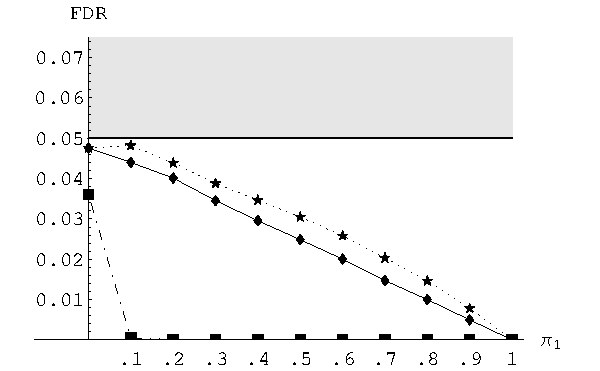
\includegraphics[width=3in]{fig_alphasim1a}
        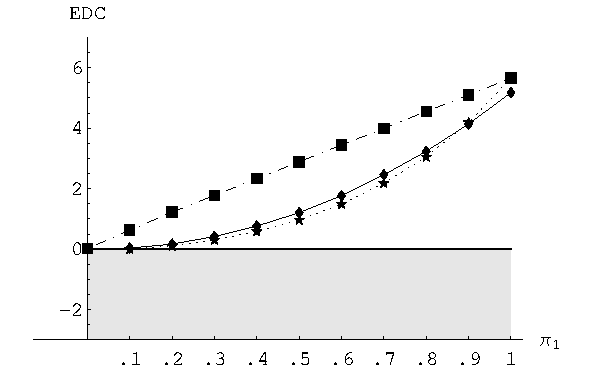
\includegraphics[width=3in]{fig_alphasim1b} }
\end{figure}


Alpha-investing guarantees protection from too many false rejections,
but how well does it find signal?  Figure \ref{fi:alphapower} compares
the power of the these alpha-investing rules to that of step-down
testing.  The plot shows the number of correct rejections
$S^\theta(m)$ made by three different rules: aggressive
alpha-investing that exploits domain knowledge 
\eqn{eq:aggressive}, conservative alpha-investing \eqn{eq:conservative}, and step-down testing.  The figure shows the average
number of hypotheses rejected by each investing rule relative to the
number rejected by step-down testing, on a percentage scale.  For
example, with a weak signal (the fraction of signal is $\pi_1 = 0.10$),
\begin{displaymath}
 100 \,\frac{S^\theta(m,\mbox{aggressive investing})}
            {S^\theta(m,\mbox{step-down})} > 150 \%
\end{displaymath}
In general, for weak signals, aggressive alpha-investing identifies
about 30\% more false hypotheses than step-down testing. The two
become more similar as signal strength grows (in the form of more
false null hypotheses).  Conservative alpha-investing rejects a few more hypothesis, about 5-10\%, than this form of step-down testing.

\begin{figure}
\caption{\label{fi:alphapower} \sl
Aggressive alpha-investing using \eqn{eq:aggressive} exploits domain
knowledge to achieve higher power than step-down testing.
This plot shows the percentage of correctly rejected null hypotheses
for each procedure, relative to step-down testing.  Both
alpha-investing rules have more power than step-down testing with the
same size.  \dpf{should this be controls FWER in the weak sense?} }

\vspace*{0.05in} 
\centerline{
            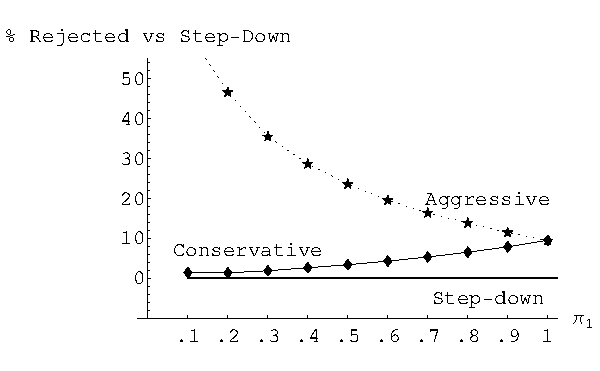
\includegraphics[width=4in]{fig_alphapower} 
           }
\end{figure}


\subsection{Comparison to Step-Down Testing}

This section discusses testing a fixed set hypothesis as a
 stream of hypothesis.  We assume that the set of hypothesis have
 no intrinsic order to them; they should all be treated symmetrically.
 Any order that is placed on them breaks this symmetry and
 favors the test of some over others.  To avoid this favoritism, we randomly order
 the hypothesis and treat them as a sequence.  This randomization
 treats them all symmetrically, but leads to an inefficient test.  Some sort of
 Rao-Blackwellization might help here, but would require
 introducing randomized tests.  This section describes a simpler solution.

To achieve the desired symmetry, we use some the ideas mentioned in
 the previous section.  We begin by investing small amounts of alpha-wealth.
  This spending policy means that we will run out of hypothesis well before we run out of alpha-wealth.  To improve the tests, however, we use this left over alpha-wealth to take a second pass through the hypotheses that were not rejected in the first pass.  Though we don't advocate this as a general procedure, it is allowed by our theorems. Gradually ``nibbling'' away at the hypotheses in this fashion produces a procedure that is similar to step-down
testing.  

Set the initial alpha-wealth $W(0) = \alpha$ and the pay-out $\omega = \alpha$.
  Define an alpha-investing rule that allocates its available alpha-wealth
 $W(j)$ equally over the hypotheses that have not been rejected, in the style of the conservative spending policy defined in \eqn{eq:conservative}.  Assume that the complete null hypothesis and that step-down testing rejects $0 < k < m$ hypotheses.  The comparable alpha-investing rule begins by testing each hypothesis in ${\cal H}(m)$ at the Bonferroni level $\alpha/m$. This first pass rejects at least one hypothesis, namely the most significant $H_{(1)}$.  To keep the presentation simple, suppose that only one hypothesis has p-value less than $\alpha/m$.  Following \eqn{eq:Wm}, the rule pays $\log(1-\alpha/m)$ for each test that it does not reject and earns $\alpha + \log(1-p_{(1)})$ for rejecting $H_{(1)}$.  Hence, after testing each hypothesis at level $\alpha/m$, its alpha-wealth is at least
\begin{eqnarray}
 W(m) 
   &=& W(0) + \alpha + \log (1-p_{(1)}) + (m-1) \log(1-\alpha/m) \cr
   &\ge& 2\alpha + m \log(1-\alpha/m)                            \cr
   &\ge& \alpha - \al^2/m
\label{eq:approx}
\end{eqnarray}
After this first pass, its alpha-wealth is virtually unchanged, and the rule retains enough wealth to reject $H_{(2)}$ if step-down testing has rejected $k > 1$ hypotheses.

For the second pass through the remaining $m-1$ null hypotheses, the
 alpha-investing rule rejects any hypothesis for which $p_j \le
 2\alpha/m$, as in step-down testing.  Because the tests used in alpha-investing must condition on $p_j > \alpha/m$, this pass requires that the level of each test of the remaining $m-1$ hypothesis be set to
\begin{displaymath}
  \pr_0\left(
   \frac{\al}{m} < p_j \le \frac{2\,\al}{m} \given p_j > \frac{\al}{m}
    \right)
   = \frac{\al}{m-\al} \;.
\end{displaymath}
The alpha-investing rule possesses enough wealth after the second round to do this because,
from \eqn{eq:approx} for $\alpha \le 1/2$,
\begin{displaymath}
    \frac{\al}{m-\al} \le \frac{\alpha - \al^2/m}{m-1} 
     \le \frac{W(m)}{m-1} \;.
\end{displaymath}
As in the first round, this second pass again approximately conserves
the alpha-wealth of the procedure.  Thus, so long as $m$ is large and
$k \ll m$ so that bounds similar to \eqn{eq:approx} hold, each
pass though the hypotheses conserves enough alpha-wealth for the next
round of tests.  In this way, the investing rule gradually raises the
threshold to the level used in step-down testing.

Instead of spending equally on each hypothesis one could weight
 each hypothesis differently.  This idea of using prior information is
 implicit in alpha-spending rules.  Recently, \cite{wasserman04} uses
 prior information on the hypotheses to come up with a weighted
 Benjamini-Hochberg (called wBH) procedure.  Following the ideas of
 this section, we can show that the wBH procedure satisfies the mFDR.

%--------------------------------------------------------------------------
\section{Discussion}           \label{sec:discussion}
%--------------------------------------------------------------------------

$\log 1/(1-p_j) \approx
p_j$ from the invested $\alpha_j$ and earns a pay-out $\omega$ that is
added to its alpha-wealth.  If $p_j > \alpha_j$, the procedure does not
reject $H_j$ and its alpha-wealth decreases by $\log(1-\alpha_j)$.
The change in the alpha-wealth is thus
\begin{equation}
  W(j) - W(j-1) =
   \left\{ \begin{array}{cc}
                \omega + \log (1-p_j) & \mbox{ if } p_j \le \alpha_j  \;,\cr
                \log(1 - \alpha_j)       & \mbox{ if } p_j > \alpha_j   \;.
           \end{array} \right.
\label{eq:Wm}
\end{equation}
If the p-value is uniformly distributed on [0,1], then the expected
 change in the alpha-wealth is $-(1 - \omega) \alpha_j$, which suggests
 alpha-wealth decreases when testing a true null hypothesis. (A section in the appendix explains the presence of logs in \eqn{eq:Wm}. The approximation $\log(1-p) \approx -p$ provides a more interpretable, nearly identical adjustment.)


Part of our motivation for alpha-investing arose in our work using stepwise
 regression for data mining \citep{fosterstine04:bank}.  In this application, we compared forward stepwise regression to tree-based classifiers for predicting the onset
of personal bankruptcy.  To make regression competitive, we expanded
the stepwise search to include all possible interactions among more
than 350 predictors.  This expansion of the scope produced more than 67,000 possible predictors.  Because so many of these predictors are interactions
(more than 98\%), it is not surprising that most of the predictors
identified by the search were interactions.  Furthermore, because of
the wide scope of this search, the procedure lacked power to find
subtle effects that while small, improve the predictive accuracy.  It became apparent to us that a hybrid search that 
considers interactions $X_j\,*\,X_k$, say, {\em only after} including
both $X_j$ and $X_k$ as main effects might be very effective.  At the
time, however, we lacked a method for controlling the variable selection when the scope of the search dynamically expands.  We expect to use alpha-investing heavily in this work in
the future.

We speculate that the greatest reward from developing a specialized
testing strategy will come from developing methods that select the
next hypothesis rather than specific functions to determine how $\alpha$
is spent.  The rule \eqn{eq:aggressive} invests most of the current
wealth in testing hypotheses following a rejection.  One can devise other choices.  Our work and those of others in information theory \citep{rissanen83, fosterstinewyner02}, however, suggest that one can find universal alpha-investing rules.  Given a
procedure for ordering the hypothesis, a universal alpha-investing
rule would lead to rejecting as many hypothesis as the best rule
within some class. We would expect such a rule to spend its
alpha-wealth a bit more slowly than the simple rule
\eqn{eq:aggressive}, but retain this general form.

Another application for alpha-investing is in group-sequential
clinical trials.  In other work \citep{fosterstine05} we address the
concept of adaptive design with a modification for alpha-investing.
We show that the complaints raised in \cite{tsiatis03} about the
efficiency of such tests can be mitigated by proper
alpha-investing.  At the same time, we allow the researcher
freedom to design rules that guide how to spend or invest their
alpha-wealth.


%--------------------------------------------------------------------------
\section*{Appendix}  
%--------------------------------------------------------------------------

\subsection*{Micro-investing}

The presence of $\log (1-\alpha)$ and $\log (1-p)$ in \eqn{eq:Wm}
 deserves some explanation.  Suppose for this discussion that an alpha-investing rule spends the level $\alpha$, which is slightly less than $-\log(1-\alpha)$, when the hypothesis is not rejected.  In this setting, consider the following
 ``micro-investment'' approach to testing a single null hypothesis
 $H_0$.  Set the initial wealth $W(0) = \alpha$. Rather than use one test at
 level $\alpha$, a micro-investment approach uses a sequence of tests,
 each risking a small amount $\ep \ll \alpha$ of the total
 alpha-wealth.   First test $H_0$ at level $\ep$; reject $H_0$ if the initial p-value of the test $p \le \ep$.  If $p > \ep$, the investing rule pays $\ep$ for the
 first test, and then tests $H_0$ conditionally on $p > \ep$ at
 level $\ep$.  This second test rejects $H_0$ if $\ep < p \le 2\ep -
 \ep^2$.  If this second test does not reject $H_0$, the investing
 rule again pays $\ep$ and retests $H_0$, now conditionally on $p >
 2\ep - \ep^2$.  This process continues until the investing rule
 either spends all of its alpha-wealth or rejects $H_0$ on the $k$th
 attempt because
\begin{displaymath}
  1-(1-\ep)^{k-1} < p \le 1-(1-\ep)^k \;.
\end{displaymath}
If the procedure rejects $H_0$ after $k$ tests, then the total
of the micro-payments made is
\begin{displaymath}
  k \,\ep \ge \frac{\log (1-p)}{\log (1-\ep)}\; \ep
  \rightarrow -\log (1-p) \mbox{ as } \ep \rightarrow 0\;.
\end{displaymath}
The increments to the wealth defined in equation \eqn{eq:Wm}
essentially treat each test as a sequence of such micro-level tests.

\subsection*{Equation \ref{eq:bounds}}
We use only the formula $1/(1+x) \le 1 - x$ and the definition $S=R-V$ to
generate bounds for the difference between mFDR and FDR.  First observe that
\begin{eqnarray*}
\delta &\equiv& mFDR_0 - FDR = E(V)/E(R) - E(V/R) \\
          & =    &  \frac{E(V)}{E(R)} - \frac{1}{E(R)}E\left(\frac{V}{1 + (R - ER)/ER)}\right) \\
          & \ge  & \frac{E(V)}{E(R)} - \frac{1}{E(R)}E(V(1 - (R - ER)/ER) \\
          & \ge  &  (1/E(R))Cov(V,R)/ER = Cov(V,R)/(ER)^2 
\end{eqnarray*}
Hence, $\delta \ge \gamma_R\rho \sigma_V/\mu_R$.
To obtain a lower bound for $\delta$,
\begin{eqnarray*}
  \delta & = & E(R-S)/E(R) - E((R-S)/R) \\
            & = & 1 - E(S)/E(R) - 1 + E(S/R) \\
            & = & E(S/R) - E(S)/E(R) \\
            & = & \frac{1}{E(R)}E\left(\frac{S}{1 + (R - ER)/ER)} - E(S)/E(R)\right) \\
            & \le&  (1/E(R))E(S(1 - (R - ER)/ER) - E(S)/E(R) \\
            & \le&  -(1/E(R))Cov(S,R)/ER = -Cov(S,R)/(ER)^2 
\end{eqnarray*}
Hence,
\begin{eqnarray*}
  \delta & \le  & -Cov(R-V,R)/(ER)^2 \\
            & = & (-\sigma^2_R + Cov(V,R))/(ER)^2
\end{eqnarray*}
As a result, $\delta \le Cov(V,R)/(ER)^2 + \gamma^2_R$.

\subsection{Proof of Theorem \ref{thm:finite:stopping}} 

First we will define the assumptions that define the class of models.

To start with, we will need an infinite sequence of hypothesis that we
 are testing.  Under this set up we can define: $S^\theta(\infty) =
 \lim_{m \to \infty} S^\theta(m)$, namely the number of correct
 rejections over the entire sequence.  We will be interested in the
 case where this is unbounded, namely, $S^\theta(\infty) = \infty$.
  If this occurs, then $T_{R=r}$ will be almost surely finite for all
 $r$.  This is state precisely as:
\begin{lemma}
If $S^\theta(\infty) = \infty$ then $T_{R=r} < \infty$ for all $r$.
\end{lemma}
{\bf Proof:}

 $R(m) \ge S^\theta(m) \to \infty$ as $m \to \infty$.  Hence, for all $r$
there exists an $T$ such that $R(T) > r$. \hfill \QED

\noindent
Note: This doesn't require that a large fraction of the hypotheses are
 non-null.  It simply means that regardless of how many hypothesis
 you have tested so far, there is always at least one more to be found
 that is significant enough that is likely that it will be found.

We will say that an alpha-investing scheme is {\em thrifty} if it
 never commits all of its current wealth to the current hypothesis.  A
 thrifty scheme will never give up the search for more signal.  It will
 always save a bit more for the future.  All the scheme that we
 consider in this paper are thrifty.

We will say that an alpha-investing scheme is {\em hopeful} if it
 always spends at least some of its wealth on the next hypothesis.  A
 hopeful and thrifty scheme will always burn at least some alpha on
 every hypothesis in an infinite sequence.

A $\theta$ which has the property that for all $m$, and all $W_m > 0$,
 the chance that the alpha-investing scheme $\cal I$ will reject at
 least one more hypothesis after time $m$ is at least $.5$ is said to
 {\em provide continuous funding for $\cal I$.}  Clearly for such a
 $\theta$ we have that $S^\theta(\infty) = \infty$.

\begin{lemma}
Assume we are testing a sequence of hypothesis where each is a test of
 whether a normal distribution has mean zero.  Let $\cal I$ be a
 thrifty and hopeful alpha-investing scheme.  Consider an infinite set
 of integers: $J \subset \cal N$, $|J| = \infty$.  Then there exists a
 $\theta$, such that $\theta_i \ne 0$ only if $i \in J$ and that it
 will provide continuous funding for $\cal I$.
\end{lemma}

{\bf proof:} 

Define $\underline{\alpha}_i$ to be the least amount that could ever
 be spent to test hypothesis $i$ by scheme $\cal I$.  Since there are
 only a finite number of possible sequences of accepts and rejects
 before time $i$, this is a minimum over a finite set.  Since our rule
 is thrifty and hopeful, we know that each element in this finite set
 is non-zero.  Hence, $\underline{\alpha}_i > 0$.

Now for each $i \in J$, pick $\theta_i$ large enough so that the power
 of a $\underline{\alpha}_i$ level test is at least .5.  Then since
 the $J$ is infinite, we know that regardless of the sequence we have
 observed, there is a .5 chance of rejecting at least one more
 hypothesis after an point. 

\hfill\QED

\noindent
We have now established the following version of Theorem
\ref{thm:finite:stopping}. 
\begin{theorem}
For any thrifty and hopeful alpha-investing scheme there exists model
such that it will be provided with continuous funding.  Under such a
condition, $T_{R=r}$ is finite almost surely.
\end{theorem}


\subsection*{Proof of Theorem \ref{th:main}}

We begin by defining the following stochastic process indexed by the
 number of hypothesis that have been tested:
\begin{displaymath}
    A(j) \equiv \alpha R(j) -  V^\theta(j)  + (1 - \eta)\alpha - W(j) \; .  
\end{displaymath}
Our main lemma shows that $A(j)$ is a sub-martingale for
 alpha-investing rules with pay-out $\omega \le \alpha$.  In other
 words we will show that $A(j)$ is ``increasing'' in the sense that
\begin{displaymath}
  E_\theta\left( A(j) \given A(j-1),\,A(j-2),\ldots, A(1)\right)
  \ge A(j-1) \;.
\end{displaymath}
Note, Theorem \ref{th:main} will uses the weaker fact that
 $E(A(j)) \ge A(0)$.  By definition $V^\theta(0) = R(0) = 0$ so that
 $A(0) = (1 - \eta)\alpha - W(0) \ge 0$ if we start with $W(0) \le
 (1 - \eta)\alpha$.  When $A(j)$ is a sub-martingale, the optional stopping
 theorem implies that for all finite stopping times $M$ that $E(A(M))
 \ge 0$.  Thus,
\begin{displaymath}
E_\theta(\alpha (R(M)+(1 - \eta)) - V^\theta(M)) =  E_\theta(W(M) + A(M) )
  \ge E_\theta(A(M))
  \ge A(0) \ge 0 \; .
\end{displaymath}
The first inequality follows because the alpha-wealth $W(j) \ge 0 \;
 [a.s.]$, and the second inequality follows from the sub-martingale
 property.  Thus,
\begin{eqnarray*}
E_\theta(V^\theta(M) - \alpha (R(M)+1 - \eta)) & \le & 0 \\
E_\theta(V^\theta(M)) & \le &  \alpha (E_\theta(R(M))+1 - \eta) \\
\frac{E_\theta(V^\theta(M))}{ E_\theta(R(M))+1 - \eta}  & \le &  \alpha\\
mFDR_\eta(M) &\le&  \alpha
\end{eqnarray*}
Thus to show Theorem \ref{th:main} all we need is the following lemma:

\begin{lemma} \label{le:martingale} Let $V^\theta(m)$ and $R(m)$
 denote the cumulative number of false rejections and the cumulative
 number of all rejections, respectively, when testing a sequence of
 null hypotheses $\{H_1,\,H_2,\,\ldots\}$ using an alpha-investing
 rule ${\cal I}_{W(0),\omega}$ with pay-out $\omega \le \alpha$, and
 cumulative alpha-wealth $W(m)$.  Then the process
\begin{eqnarray*}
    A(j) 
  &\equiv& \alpha R(j) - V^\theta(j) + \alpha(1 - \eta)  - W(j) 
\end{eqnarray*}
is a sub-martingale,
\begin{equation}
   E \left(A(m) \given A(m-1), \ldots, A(1)\right) \ge A(m-1) \;.
 \label{eq:super}
\end{equation}
\end{lemma}

\noindent 
{\bf Proof.} 

We begin with some notation for the increments that define the counts
in Table \ref{ta:notation}.  Write $V^\theta(m)$ and $R(m)$ as sums of
indicators $V^\theta_j,\, R_j \in \{0,1\}$,
\begin{displaymath}
   V^\theta(m) = \sum_{j=1}^m V^\theta_j \;, \qquad
   R(m) = \sum_{j=1}^m R_j \;.
\label{eq:sums}
\end{displaymath}
Similarly write the accumulated alpha-wealth $W(m)$ and $A(m)$ as sums of
increments, $W(m) = \sum_{j=0}^m W_j$ and $A(m) = \sum_{j=0}^m A_j$.
Let $\alpha_j$ denote the alpha level of the test of $H_j$ that satisfies
the condition \eqn{eq:alpham}.  The change in the alpha-wealth from
testing $H_j$ can be written as:
\begin{displaymath}
  W_j  =  R_j \omega + \log(1 - (p_j \wedge \alpha_j))  \;,
\end{displaymath}
where $\wedge$ is the minimum operator.  Substituting this into $A_j$ we get
\begin{displaymath}
   A_j  =  (1 -\gamma -\omega) R_j - V^\theta_j  - \log(1 - (p_j \wedge
\alpha_j))  \;.
\end{displaymath}
Since $R_j \ge 0$ and $1-\gamma - \omega \ge 0$ by the conditions of the
lemma, it follows that
\begin{equation}
\label{eq:a:bound}
A_j  \ge   - V^\theta_j  - \log(1 - (p_j \wedge \alpha_j))  \;.
\end{equation}
If $\theta_j \not\in H_j$, then $V^\theta_j = 0$ and $A_j \ge 0$
almost surely.  So we only need to consider the case in which the null
hypothesis $H_j$ is true.

Abbreviate the conditional expectation
\begin{displaymath}
  E_\theta^{j-1}(X) 
     = E_\theta \left(X \given  A(1),\,A(2),\,\ldots,A(j-1) \right)\;.
\end{displaymath}
Then, when $H_j$ is true, $p_j \sim U[0,1]$ so that
\begin{eqnarray*}
  E_\theta^{j-1}(-\log(1 - (p_j \wedge \alpha_j)) 
   &=&  -\int_0^1 \log(1 - (p \wedge \alpha_j)) dp \cr
   &=&  -\int_0^{\alpha_j} \log(1 - p) dp - \int_{\alpha_j}^1 \log(1 - \alpha_j) dp \\
%  &=&  \left(-\alpha_j - (1-\alpha_j)\log(1-\alpha_j)\right) + (1-\alpha_j)\log(1-\alpha_j)\\
   &=&  \alpha_j  \;.
\end{eqnarray*}
Since $E_\theta^{j-1}(V^\theta_j) \le \alpha_j$ by the definition of
this being an $\alpha_j$ level test, equation (\ref{eq:a:bound})
implies $E_\theta^{j-1} \; A_j \ge 0$.

\hfill \QED

%--------------------------------------------------------------------------
% References
%--------------------------------------------------------------------------

\bibliography{../stat}
\bibliographystyle{../bst/rss}

\end{document} %==========================================================
